
\vspace{-2em}
\section{引言}
\label{sec:intro}
\vspace{-1em}

\begin{figure*}[t]
    \centering
\vspace{-3mm}
    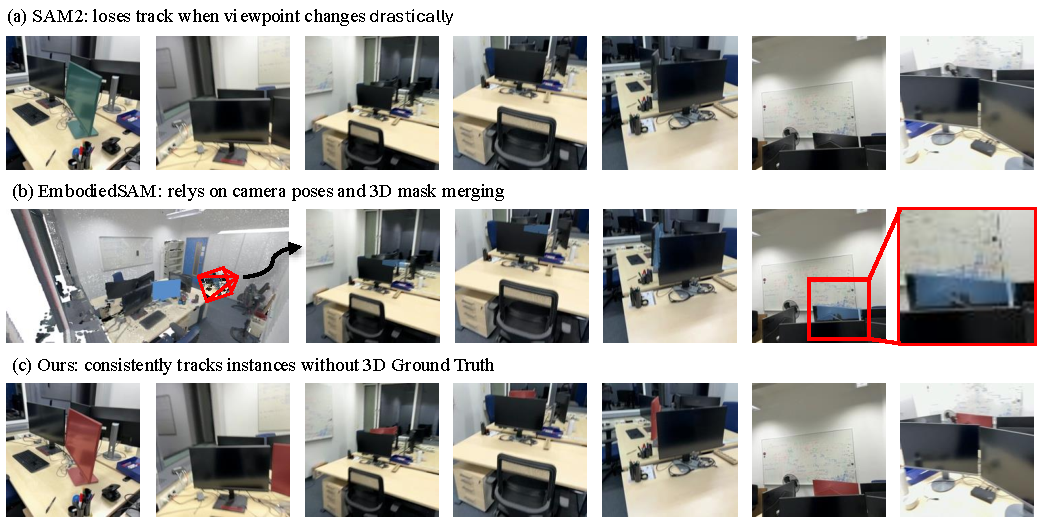
\includegraphics[width=\textwidth]{figs/comparison-teaser.pdf}
\vspace{-6mm}
    \caption{\textbf{传统 VOS 与 3D 分割方法的局限，以及我们能力的概览。}  
    (a) SAM2~\cite{ravi2024sam2} 等传统 VOS 方法在相机发生大幅视角变化时会丢失目标，导致掩码漂移或消失。  
    (b) 3D 分割方法依赖精确相机位姿和显式 3D 掩码合并；当 3D 重建不完整或噪声较大时，它们常会传播错误。  
    (c) 我们的 \textbf{3AM} 无需相机位姿或 3D 真值掩码，即可在剧烈视角变化下持续跟踪对象实例，展示了仅依靠几何感知 2D 跟踪实现鲁棒跨视角对应的能力。
    }
    \label{fig:intro-comparison}
\vspace{-3mm}
\end{figure*}

视频对象分割（VOS）旨在识别并跟踪视频序列中的目标对象，并在各帧之间保持一致的掩码。这是自动驾驶、机器人、增强现实和视频编辑等任务的基础。一个核心挑战是在大幅视角变化、短暂消失或相似干扰物存在时保持对象身份。传统 VOS 方法依赖 2D 外观特征，当对象从不同视角呈现出显著差异时容易失败。对于动态 3D 环境中的具身 AI 而言，跨多样视角持续识别对象是鲁棒场景理解的关键。

近期视频对象分割进展主要沿两条路线展开。第一类是带有记忆架构的 2D 基础模型：SAM2~\cite{ravi2024sam2} 引入了具有流式记忆和时空注意力的可提示分割。SAM2Long~\cite{ding2024sam2long} 使用记忆树保持长程身份，DAM4SAM~\cite{videnovic2025distractor} 则引入干扰物感知更新。然而，纯 2D 方法在大幅视角变化下会失败，因为外观特征无法建立可靠对应。第二类是 3D 实例分割方法：Mask3D~\cite{schult2022mask3d} 和 OneFormer3D~\cite{kolodiazhnyi2024oneformer3d} 等以提议为中心的方法在点云上运行，而 Open3DIS~\cite{nguyen2024open3dis}、SAM3D~\cite{yang2023sam3d} 和 SAM2Object~\cite{zhao2025sam2object} 等基于投影的方法将 2D 掩码提升到 3D。这些方法需要相机位姿、深度图、预处理，并具有超线性的计算扩展成本。

两种范式都存在关键缺口（\cref{fig:intro-comparison}）。SAM2 等 2D 方法效率高，但缺乏几何感知能力，在视角变化下会失败（\cref{fig:intro-comparison}a）。MOSEv2~\cite{ding2025mosev2} 表明宽基线变化会带来显著性能下降。相反，3D 方法一致性更好，但需要显式 3D 输入（\cref{fig:intro-comparison}b）且泛化困难。2D 到 3D 的提升会受到视角不一致预测的影响~\cite{jia2024sceneverse,peng2023openscene,takmaz2023openmask3d,xu2024embodiedsam,zhao2025sam2object}。PanSt3R~\cite{zust2025panst3r} 等端到端方法需要离线处理。\emph{能否在不使用显式 3D 监督的情况下，同时保持可提示性和效率，实现 3D 感知、视角鲁棒的分割？}（\cref{fig:intro-comparison}c）

我们提出 \textbf{3AM}（\cref{teaser}），一种通用的 3D 感知跟踪器。核心洞察是，MUSt3R~\cite{cabon2025must3r} 通过从多视角一致性中学习到的特征编码了隐式几何对应关系。通过轻量级 Feature Merger 将多层级 MUSt3R 特征与 SAM2 的外观特征融合，我们使模型能够基于空间位置进行几何一致识别；推理时仅需 RGB 输入和用户提示。我们还提出视场感知采样策略，确保训练期间帧之间观察到空间一致的对象区域。在具有宽基线运动的 ScanNet++~\cite{yeshwanth2023scannet++} 和 Replica~\cite{replica19arxiv} 上，3AM 达到 90.6\% IoU 和 71.7\% Positive IoU，而 SAM2Long 分别为 74.7\% 和 41.3\%（提升 +15.9 和 +30.4 个百分点）。

总之，我们的贡献如下：
\begin{itemize}
\item \textbf{关于 2D 跟踪与 3D 一致性差距的关键观察。}
2D 跟踪在大幅视角变化下存在根本限制。现有 3D 方法需要相机位姿、深度或 3D 掩码，而这些在实践中通常不可得。这促使我们提出几何感知框架，在推理时无需 3D 监督即可实现跨视角一致性。
\item \textbf{一种 3D 感知特征整合框架}，将 3D 重建模型的几何特征与 SAM2 的外观特征融合；以及 \textbf{一种视场感知训练策略}，通过保证几何一致性来有效学习 3D 对应关系。
\item \textbf{一种通用跟踪框架}，可对非刚性或高度动态对象自适应回退到原始 SAM2；同时通过 \textbf{广泛实验评估} 证明，在 ScanNet++ 和 Replica 等挑战性数据集上，尤其在对象重现和显著视角变化场景中，我们相较最先进 VOS 方法取得一致提升，并在常规 VOS 基准上保持有竞争力的性能。
\end{itemize}
